%%%%%%%%%%%%%%%%%%%%%%%%%%%%%%%%%%%%%%%%%%%%%%%%%%%%%%%%%%%%%%%%%%%%%%
% CS2100 Midterms Cheatsheet
% Author: San Diego John Michael Bautista
%%%%%%%%%%%%%%%%%%%%%%%%%%%%%%%%%%%%%%%%%%%%%%%%%%%%%%%%%%%%%%%%%%%%%%

\documentclass[10pt,landscape]{article}
\usepackage{amssymb,amsmath,amsthm,amsfonts}
\usepackage{multicol,multirow}
\usepackage{calc}
\usepackage{ifthen}
\usepackage[landscape]{geometry}
\usepackage[colorlinks=true,citecolor=blue,linkcolor=blue]{hyperref}
\usepackage{mdframed}
\usepackage{graphicx}
\graphicspath{ {./images/} }


\ifthenelse{\lengthtest { \paperwidth = 11in}}
{ \geometry{top=.5in,left=.5in,right=.5in,bottom=.5in} }
{\ifthenelse{ \lengthtest{ \paperwidth = 297mm}}
    {\geometry{top=1cm,left=1cm,right=1cm,bottom=1cm} }
    {\geometry{top=1cm,left=1cm,right=1cm,bottom=1cm} }
}
\pagestyle{empty}
\makeatletter
\renewcommand{\section}{\@startsection{section}{1}{0mm}%
    {-1ex plus -.5ex minus -.2ex}%
    {0.5ex plus .2ex}%x
    {\normalfont\large\bfseries}}
\renewcommand{\subsection}{\@startsection{subsection}{2}{0mm}%
    {-1explus -.5ex minus -.2ex}%
    {0.5ex plus .2ex}%
    {\normalfont\normalsize\bfseries}}
\renewcommand{\subsubsection}{\@startsection{subsubsection}{3}{0mm}%
    {-1ex plus -.5ex minus -.2ex}%
    {1ex plus .2ex}%
    {\normalfont\small\bfseries}}
\makeatother
\setcounter{secnumdepth}{0}
\setlength{\parindent}{0pt}
\setlength{\parskip}{0pt plus 0.5ex}

% -----------------------------------------------------------------------

\title{CS2100 Midterms CheatSheet}

\begin{document}

\raggedright
\footnotesize

\begin{center}
    \Large{\textbf{CS2100 Midterms Cheatsheet}} \\
\end{center}
\begin{multicols}{3}
    \setlength{\premulticols}{1pt}
    \setlength{\postmulticols}{1pt}
    \setlength{\multicolsep}{1pt}
    \setlength{\columnsep}{2pt}

    \begin{mdframed}
        \section{12. Processor Control}
    \end{mdframed}

    % -----------------------------------------------------------------------
    % CONTROL SIGNALS Lecture 12
    % -----------------------------------------------------------------------

    \subsection{Control Signals}
    \begin{itemize}
        \item \textbf{RegDst} - (@Decode/OperandFetch) Selects the destination of WriteRegister in register file
              \begin{itemize}
                  \item 0/1: WriteRegister = Ins[20:16] (rt) / Inst[15:11] (rd / immediate)
              \end{itemize}
        \item \textbf{RegWrite} - (@Decode/OperandFetch) Indicates if writing on WriteRegister is enabled
              \begin{itemize}
                  \item 0/1: No register write / WD write to WR
              \end{itemize}
        \item \textbf{ALUSrc} - (@ALU) Determines the 2nd ALU input
              \begin{itemize}
                  \item 0/1: Read Data 2 / SignExtend(Inst15:0) (Sign extended Immediate)
              \end{itemize}
        \item \textbf{ALUcontrol} - (@ALU) Determines the type of operation to execute
              \begin{itemize}
                  \item 0000: AND
                  \item 0001: OR
                  \item 0010: add
                  \item 0110: subtract
                  \item 0111: slt
                  \item 1100: NOR
              \end{itemize}
        \item \textbf{MemRead} - (@Memory) Indicates if read from memory using Address returned by ALU
              \begin{itemize}
                  \item 0/1: No read / Reads memory with Address returned by ALU
              \end{itemize}
        \item \textbf{MemWrite} - (@Memory) Indicates if write to memory using RD2 of Register File
              \begin{itemize}
                  \item 0/1: No memory write / Writes RD2 into the memory in Address returned by ALU
              \end{itemize}
        \item \textbf{MemToReg} - (@RegWrite) Indicates which one to write back into WriteData in register file
              \begin{itemize}
                  \item 0/1: WriteData = ALU result / Memory read data
              \end{itemize}
        \item \textbf{PCSrc} - (@ALU) Indicates whether to take branch address or not
              \begin{itemize}
                  \item 0/1: \(PC = PC\) + 4 / \(PC = SignExt(Inst[15:0]) << 2 + (PC + 4)\)
                  \item PCSrc = isBranch AND isZero
              \end{itemize}
    \end{itemize}


    \subsection{ALU}
    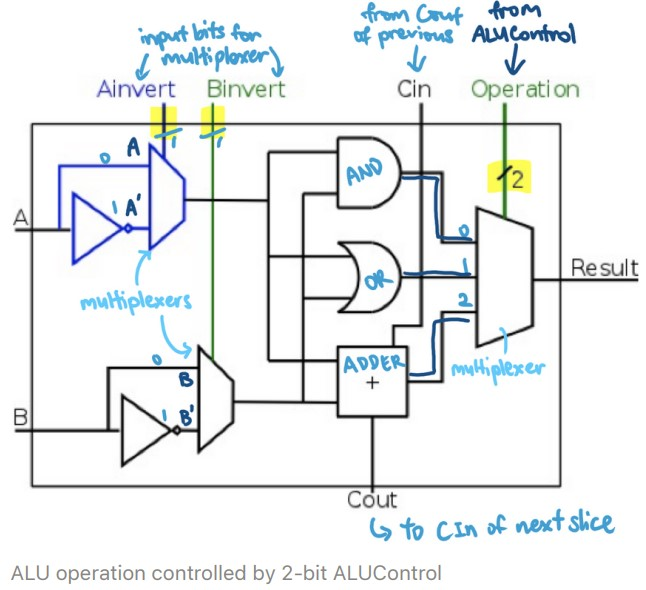
\includegraphics[width=\linewidth]{alu_diagram}
    \textit{* Note: operation is determined by the last 2-bits}
    \textit{* Subtraction has Cin = 1 for bit-0}

    \subsection{Multilevel Decoding}
    Used to generate the ALUcontrol signal. \textit{(Simpler and more efficient design than Brute Force approach)}
    \begin{enumerate}
        \item Generate a 2-bit ALUop signal from opcode
        \item Use ALUop and Function code (for R-type) to generate 4-bit ALUcontrol signal
    \end{enumerate}
    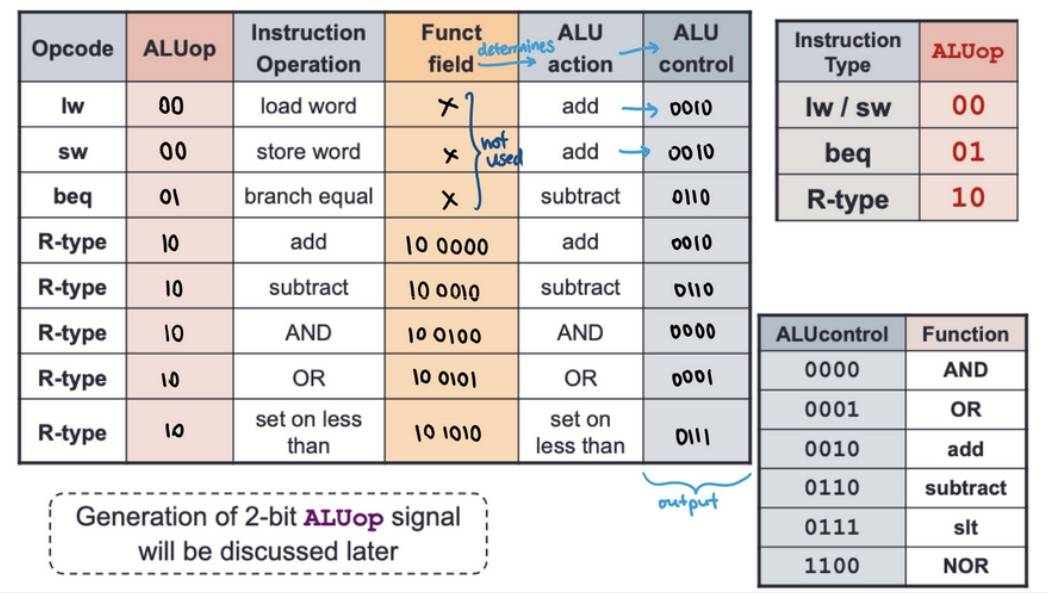
\includegraphics[width=\linewidth]{alu_generate_table}
    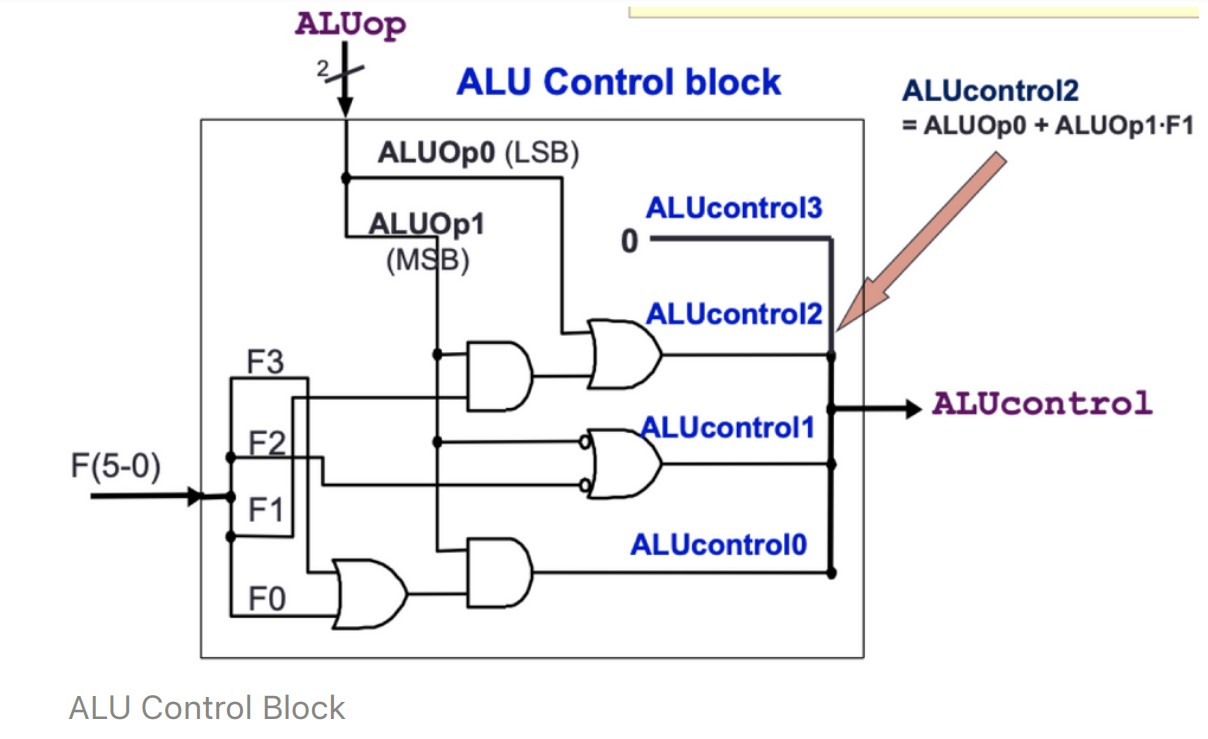
\includegraphics[width=\linewidth]{alu_control_block}

    \subsection{Control Combinational Circuit}
    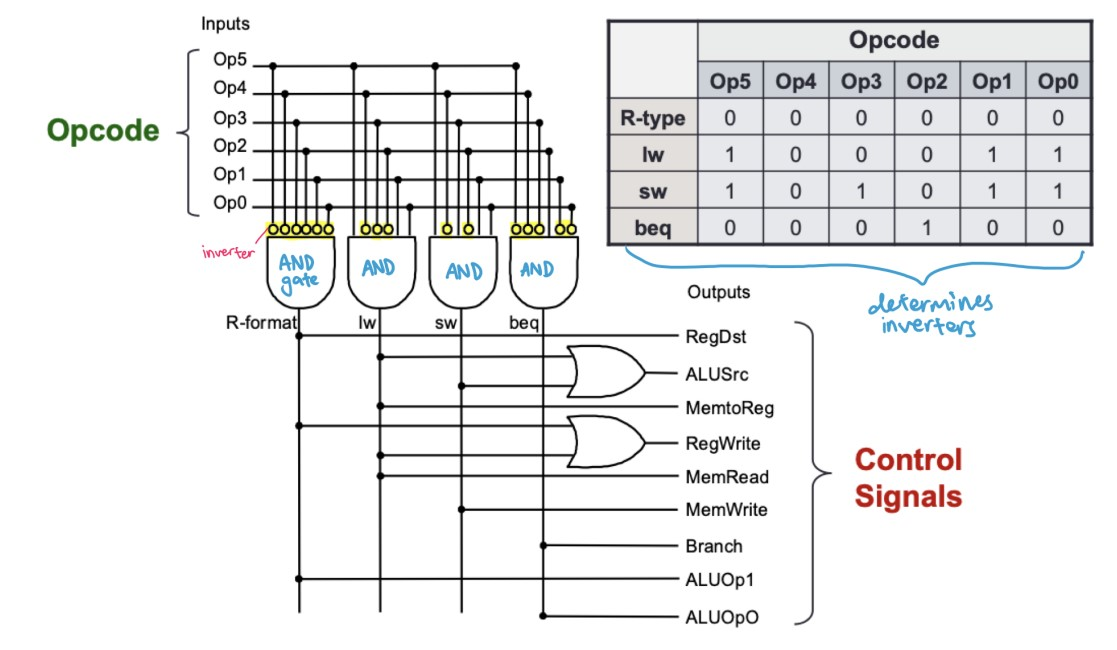
\includegraphics[width=\linewidth]{combinational_circuit}

    \subsection{Instruction Execution}
    How the implementation of fetch, decode, memory, write, etc. are actually done

    Mainly three things:
    \begin{enumerate}
        \item Read contents from register / memory
        \item Perform some form of computation
        \item Write results to register / memory
    \end{enumerate}

    \subsubsection{Single Cycle Execution}
    All performed within a clock period.\newline
    \textbf{disadvantage:} all instructions will take the same time as the slowest one.
    \subsubsection{Multi Cycle Execution}
    Break up instructions into execution steps (Fetch, Decode, ALU Operation, Mem read/write, Register Write).
    Each execution is one clock cycle.
    \textbf{disadvantage:} time taken depends on instructions and may not necessarily be faster.


    \section{Spaces and new lines}

    \LaTeX\ ignores extra spaces and new lines. For example,

    \verb!This   sentence will       look!

    \verb!fine after      it is     compiled.!

    This   sentence will       look
    fine after      it is     compiled.


    Leave one full empty line between two paragraphs. Place \verb!\\! at the end of a line to create a new line (but not create a new paragraph).

    \verb!This!

    \verb!compiles!

    ~

    \verb!like\\!

    \verb!this.!

    This
    compiles

    like\\
    this.

    Use  \verb!\noindent! to prevent a paragraph from indenting.

    \section{Comments}

    Use \verb!%! to create a comment. Nothing on the line after the \verb!%! will be typeset. \verb!$f(x)=\sin(x)$ %this is the sine function! yields $f(x)=\sin(x)$%this is the sine function

    \section{Delimiters}

    \begin{tabular}{lll}
        \emph{description} & \emph{command} & \emph{output} \\
        parentheses        & \verb!(x)!     & (x)           \\
        brackets           & \verb![x]!     & [x]           \\
        curly braces       & \verb!\{x\}!   & \{x\}         \\
    \end{tabular}

    To make your delimiters large enough to fit the content, use them together with \verb!\right! and \verb!\left!. For example, \verb!\left\{\sin\left(\frac{1}{n}\right)\right\}_{n}^! \verb!{\infty}! produces\\ $\displaystyle \left\{\sin\left(\frac{1}{n}\right)\right\}_{n}^{\infty}$.

    Curly braces are non-printing characters that are used to gather text that has more than one character. Observe the differences between the four expressions \verb!x^2!, \verb!x^{2}!, \verb!x^2t!, \verb!x^{2t}! when typeset: $x^2$, $x^{2}$, $x^2t$, $x^{2t}$.


    \section{Lists}

    You can produce ordered and unordered lists.

    \begin{tabular}{lll}
        \emph{description}          & \emph{command} & \emph{output} \\
        unordered list              &
        \begin{tabular}{l}
            \verb!\begin{itemize}! \\
            \verb!  \item!         \\
            \verb!  Thing 1!       \\
            \verb!  \item!         \\
            \verb!  Thing 2!       \\
            \verb!\end{itemize}!
        \end{tabular}   &
        \begin{tabular}{l}
            $\bullet$ Thing 1 \\
            $\bullet$ Thing 2
        \end{tabular}                                            \\
        ~                                                            \\
        ordered list                &
        \begin{tabular}{l}
            \verb!\begin{enumerate}! \\
            \verb!  \item!           \\
            \verb!  Thing 1!         \\
            \verb!  \item!           \\
            \verb!  Thing 2!         \\
            \verb!\end{enumerate}!
        \end{tabular} &
        \begin{tabular}{l}
            1.~Thing 1 \\
            2.~Thing 2
        \end{tabular}
    \end{tabular}


    \section{Symbols (in \emph{math} mode)}

    \subsection{The basics}
    \begin{tabular}{lll}
        \emph{description}       & \emph{command}      & \emph{output}   \\
        addition                 & \verb!+!            & $+$             \\
        subtraction              & \verb!-!            & $-$             \\
        plus or minus            & \verb!\pm!          & $\pm$           \\
        multiplication (times)   & \verb!\times!       & $\times$        \\
        multiplication (dot)     & \verb!\cdot!        & $\cdot$         \\
        division symbol          & \verb!\div!         & $\div$          \\
        division (slash)         & \verb!/!            & $/$             \\
        circle plus              & \verb!\oplus!       & $\oplus$        \\
        circle times             & \verb!\otimes!      & $\otimes$       \\
        equal                    & \verb!=!            & $=$             \\
        not equal                & \verb!\ne!          & $\ne$           \\
        less than                & \verb!<!            & $<$             \\
        greater than             & \verb!>!            & $>$             \\
        less than or equal to    & \verb!\le!          & $\le$           \\
        greater than or equal to & \verb!\ge!          & $\ge$           \\
        approximately equal to   & \verb!\approx!      & $\approx$       \\
        infinity                 & \verb!\infty!       & $\infty$        \\
        dots                     & \verb!1,2,3,\ldots! & $1,2,3,\ldots$  \\
        dots                     & \verb!1+2+3+\cdots! & $1+2+3+\cdots$  \\
        fraction                 & \verb!\frac{a}{b}!  & $\frac{a}{b}$   \\
        square root              & \verb!\sqrt{x}!     & $\sqrt{x}$      \\
        $n$th root               & \verb!\sqrt[n]{x}!  & $\sqrt[n]{x}$   \\
        exponentiation           & \verb!a^b!          & $a^{b}$         \\
        subscript                & \verb!a_b!          & $a_{b}$         \\
        absolute value           & \verb!|x|!          & $|x|$           \\
        natural log              & \verb!\ln(x)!       & $\ln(x)$        \\
        logarithms               & \verb!\log_{a}b!    & $\log_{a}b$     \\
        exponential function     & \verb!e^x=\exp(x)!  & $e^{x}=\exp(x)$ \\
        degree                   & \verb!\deg(f)!      & $\deg(f)$       \\
    \end{tabular}
    \newpage

    \subsection{Functions}
    \begin{tabular}{lll}
        \emph{description} & \emph{command}       & \emph{output}                                                                 \\
        maps to            & \verb!\to!           & $\to$                                                                         \\
        composition        & \verb!\circ!         & $\circ$                                                                       \\
        piecewise          & \verb!|x|=!          & \multirow{5}{*}{$\displaystyle |x|=\begin{cases}x&x\ge 0\\-x&x<0\end{cases}$} \\
        function           & \verb!\begin{cases}! &                                                                               \\
                           & \verb!x & x\ge 0\\!  &                                                                               \\
                           & \verb!-x & x<0!      &                                                                               \\
                           & \verb!\end{cases}!   &
    \end{tabular}

    \subsection{Greek and Hebrew letters}
    \begin{tabular}{llll}
        \emph{command}     & \emph{output} & \emph{command}  & \emph{output} \\
        \verb!\alpha!      & $\alpha$      & \verb!\tau!     & $\tau$        \\
        \verb!\beta!       & $\beta$       & \verb!\theta!   & $\theta$      \\
        \verb!\chi!        & $\chi$        & \verb!\upsilon! & $\upsilon$    \\
        \verb!\delta!      & $\delta$      & \verb!\xi!      & $\xi$         \\
        \verb!\epsilon!    & $\epsilon$    & \verb!\zeta!    & $\zeta$       \\
        \verb!\varepsilon! & $\varepsilon$ & \verb!\Delta!   & $\Delta$      \\
        \verb!\eta!        & $\eta$        & \verb!\Gamma!   & $\Gamma$      \\
        \verb!\gamma!      & $\gamma$      & \verb!\Lambda!  & $\Lambda$     \\
        \verb!\iota!       & $\iota$       & \verb!\Omega!   & $\Omega$      \\
        \verb!\kappa!      & $\kappa$      & \verb!\Phi!     & $\Phi$        \\
        \verb!\lambda!     & $\lambda$     & \verb!\Pi!      & $\Pi$         \\
        \verb!\mu!         & $\mu$         & \verb!\Psi!     & $\Psi$        \\
        \verb!\nu!         & $\nu$         & \verb!\Sigma!   & $\Sigma$      \\
        \verb!\omega!      & $\omega$      & \verb!\Theta!   & $\Theta$      \\
        \verb!\phi!        & $\phi$        & \verb!\Upsilon! & $\Upsilon$    \\
        \verb!\varphi!     & $\varphi$     & \verb!\Xi!      & $\Xi$         \\
        \verb!\pi!         & $\pi$         & \verb!\aleph!   & $\aleph$      \\
        \verb!\psi!        & $\psi$        & \verb!\beth!    & $\beth$       \\
        \verb!\rho!        & $\rho$        & \verb!\daleth!  & $\daleth$     \\
        \verb!\sigma!      & $\sigma$      & \verb!\gimel!   & $\gimel$
    \end{tabular}


    \subsection{Set theory}
    \begin{tabular}{lll}
        \emph{description}           & \emph{command}               & \emph{output}                           \\
        set brackets                 & \verb!\{1,2,3\}!             & $\{1,2,3\}$                             \\
        element of                   & \verb!\in!                   & $\in$                                   \\
        not an element of            & \verb!\not\in!               & $\not\in$                               \\
        subset of                    & \verb!\subset!               & $\subset$                               \\
        subset of                    & \verb!\subseteq!             & $\subseteq$                             \\
        not a subset of              & \verb!\not\subset!           & $\not\subset$                           \\
        contains                     & \verb!\supset!               & $\supset$                               \\
        contains                     & \verb!\supseteq!             & $\supseteq$                             \\
        union                        & \verb!\cup!                  & $\cup$                                  \\
        intersection                 & \verb!\cap!                  & $\cap$                                  \\
        big union                    &
        \verb!\bigcup_{n=1}^{10}A_n! &
        $\displaystyle \bigcup_{n=1}^{10}A_{n}$                                                               \\
        big intersection             & \verb!\bigcap_{n=1}^{10}A_n! & $\displaystyle \bigcap_{n=1}^{10}A_{n}$ \\
        empty set                    & \verb!\emptyset!             & $\emptyset$                             \\
        power set                    & \verb!\mathcal{P}!           & $\mathcal{P}$                           \\
        minimum                      & \verb!\min!                  & $\min$                                  \\
        maximum                      & \verb!\max!                  & $\max$                                  \\
        supremum                     & \verb!\sup!                  & $\sup$                                  \\
        infimum                      & \verb!\inf!                  & $\inf$                                  \\
        limit superior               & \verb!\limsup!               & $\limsup$                               \\
        limit inferior               & \verb!\liminf!               & $\liminf$                               \\
        closure                      & \verb!\overline{A}!          & $\overline{A}$
    \end{tabular}

    \subsection{Calculus}
    \begin{tabular}{lll}
        \emph{description}                              & \emph{command}                                & \emph{output}                      \\
        derivative                                      & \verb!\frac{df}{dx}!                          & $\displaystyle \frac{df}{dx}$      \\
        derivative                                      & \verb!\f'!                                    & $f'$                               \\
        partial derivative                              &
        \begin{tabular}{l}
            \verb!\frac{\partial f}! \\ \verb!{\partial x}!
        \end{tabular} & $\displaystyle \frac{\partial f}{\partial x}$                                                                        \\
        integral                                        & \verb!\int!                                   & $\displaystyle\int$                \\
        double integral                                 & \verb!\iint!                                  & $\displaystyle\iint$               \\
        triple integral                                 & \verb!\iiint!                                 & $\displaystyle\iiint$              \\
        limits                                          & \verb!\lim_{x\to \infty}!                     & $\displaystyle \lim_{x\to \infty}$ \\
        summation                                       &
        \verb!\sum_{n=1}^{\infty}a_n!                   &
        $\displaystyle \sum_{n=1}^{\infty}a_n$                                                                                               \\
        product                                         &
        \verb!\prod_{n=1}^{\infty}a_n!                  &
        $\displaystyle \prod_{n=1}^{\infty}a_n$
    \end{tabular}




    \subsection{Logic}
    \begin{tabular}{lll}
        \emph{description}  & \emph{command}         & \emph{output}     \\
        not                 & \verb!\sim!            & $\sim$            \\
        and                 & \verb!\land!           & $\land$           \\
        or                  & \verb!\lor!            & $\lor$            \\
        if...then           & \verb!\to!             & $\to$             \\
        if and only if      & \verb!\leftrightarrow! & $\leftrightarrow$ \\
        logical equivalence & \verb!\equiv!          & $\equiv$          \\
        therefore           & \verb!\therefore!      & $\therefore$      \\
        there exists        & \verb!\exists!         & $\exists$         \\
        for all             & \verb!\forall!         & $\forall$         \\
        implies             & \verb!\Rightarrow!     & $\Rightarrow$     \\
        equivalent          & \verb!\Leftrightarrow! & $\Leftrightarrow$
    \end{tabular}

    \subsection{Linear algebra}
    \begin{tabular}{lll}
        \emph{description}           & \emph{command}              & \emph{output}                  \\
        vector                       & \verb!\vec{v}!              & $\vec{v}$                      \\
        vector                       & \verb!\mathbf{v}!           & $\mathbf{v}$                   \\
        norm                         & \verb!||\vec{v}||!          & $||\vec{v}||$                  \\
        matrix                       &
        \begin{tabular}{l}
            \verb!\left[!             \\
            \verb!\begin{array}{ccc}! \\
            \verb!1 & 2 & 3 \\!       \\
            \verb!4 & 5 & 6\\!        \\
            \verb!7 & 8 & 0!          \\
            \verb!\end{array}!        \\
            \verb!\right]!\end{tabular} &
        $\displaystyle \left[\begin{array}{ccc}1 & 2 & 3 \\4 & 5 & 6 \\7 & 8 & 0\end{array}\right]$ \\
        \\determinant&
        \begin{tabular}{l}
            \verb!\left|!             \\
            \verb!\begin{array}{ccc}! \\
            \verb!1 & 2 & 3 \\!       \\
            \verb!4 & 5 & 6 \\!       \\
            \verb!7 & 8 & 0!          \\
            \verb!\end{array}!        \\
            \verb!\right|!
        \end{tabular} &
        $\displaystyle \left|\begin{array}{ccc}1 & 2 & 3 \\4 & 5 & 6 \\7 & 8 & 0\end{array}\right|$ \\
        determinant                  & \verb!\det(A)!              & $ \det(A)$                     \\
        trace                        & \verb!\operatorname{tr}(A)! & $\operatorname{tr}(A)$         \\
        dimension                    & \verb!\dim(V)!              & $\dim(V)$                      \\
    \end{tabular}

    \subsection{Number theory}
    \begin{tabular}{lll}
        \emph{description}      & \emph{command}            & \emph{output}        \\
        divides                 & \verb!|!                  & $|$                  \\
        does not divide         & \verb!\not |!             & $\not |$             \\
        div                     & \verb!\operatorname{div}! & $\operatorname{div}$ \\
        mod                     & \verb!\mod!               & $\operatorname{mod}$ \\
        greatest common divisor & \verb!\gcd!               & $\gcd$               \\
        ceiling                 & \verb!\lceil x \rceil!    & $\lceil x\rceil$     \\
        floor                   & \verb!\lfloor x \rfloor!  & $\lfloor x \rfloor$  \\
    \end{tabular}




    \subsection{Geometry and trigonometry}
    \begin{tabular}{lll}
        \emph{description} & \emph{command}       & \emph{output}   \\
        angle              & \verb!\angle ABC!    & $\angle ABC$    \\
        degree             & \verb!90^{\circ}!    & $90^{\circ}$    \\
        triangle           & \verb!\triangle ABC! & $\triangle ABC$ \\
        segment            & \verb!\overline{AB}! & $\overline{AB}$ \\
        sine               & \verb!\sin!          & $\sin$          \\
        cosine             & \verb!\cos!          & $\cos$          \\
        tangent            & \verb!\tan!          & $\tan$          \\
        cotangent          & \verb!\cot!          & $\cot$          \\
        secant             & \verb!\sec!          & $\sec$          \\
        cosecant           & \verb!\csc!          & $\csc$          \\
        inverse sine       & \verb!\arcsin!       & $\arcsin$       \\
        inverse cosine     & \verb!\arccos!       & $\arccos$       \\
        inverse tangent    & \verb!\arctan!       & $\arctan$       \\
    \end{tabular}

    \section{Symbols (in \emph{text} mode)}

    The followign symbols do \textbf{not} have to be surrounded by dollar signs.

    \begin{tabular}{lll}
        \emph{description} & \emph{command}        & \emph{output}  \\
        dollar sign        & \verb!\$!             & \$             \\
        percent            & \verb!\%!             & \%             \\
        ampersand          & \verb!\&!             & \&             \\
        pound              & \verb!\#!             & \#             \\
        backslash          & \verb!\textbackslash! & \textbackslash \\
        left quote marks   & \verb!``!             & ``             \\
        right quote marks  & \verb!''!             & ''             \\
        single left quote  & \verb!`!              & `              \\
        single right quote & \verb!'!              & '              \\
        hyphen             & \verb!X-ray!          & X-ray          \\
        en-dash            & \verb!pp. 5--15!      & pp. 5--15      \\
        em-dash            & \verb!Yes---or no?!   & Yes---or no?
    \end{tabular}

    \section{Resources}
    Great symbol look-up site: \href{http://detexify.kirelabs.org/}{Detexify}\\
    \href{http://amath.colorado.edu/documentation/LaTeX/Symbols.pdf}{\LaTeX\ Mathematical Symbols}\\
    \href{ftp://tug.ctan.org/pub/tex-archive/info/symbols/comprehensive/symbols-letter.pdf}{The Comprehensive \LaTeX\ Symbol List}\\
    \href{http://mirrors.med.harvard.edu/ctan/info/lshort/english/lshort.pdf}{The Not So Short Introduction to \LaTeX\ 2$\varepsilon$}\\
    \href{http://www.tug.org/}{TUG: The \TeX\ Users Group}\\
    \href{http://www.ctan.org/}{CTAN: The Comprehensive \TeX\ Archive Network}\\
    ~\\
    \LaTeX\ for the Mac: \href{http://www.tug.org/mactex/}{Mac\TeX}\\
    \LaTeX\ for the PC: \href{http://www.texniccenter.org/}{{\TeX}nicCenter} and \href{http://miktex.org/}{MiK\TeX}\\
    \LaTeX\ online: \href{http://www.writelatex.com/}{WriteLaTeX}.
    \vfill
    \hrule
    ~\\
    Dave Richeson, Dickinson College, \href{http://divisbyzero.com/}{http://divisbyzero.com/}
\end{multicols}

\end{document}
